\chapter{Student tasks questionnaire}

\begin{figure}[h]
\centering
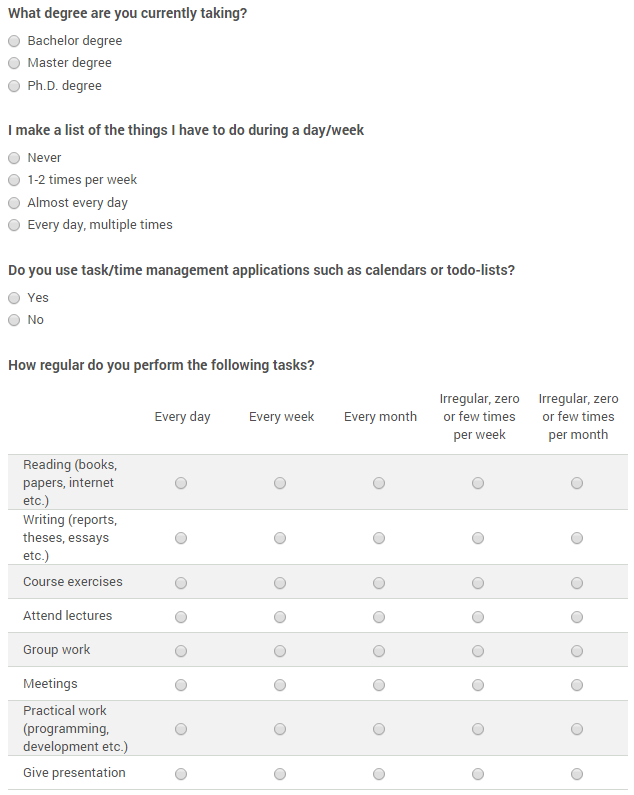
\includegraphics[width=0.8\columnwidth]{appendix/StudentTasks1.PNG}
\caption{Student tasks questionnaire part 1.}
\end{figure}

\begin{figure}[h]
\centering
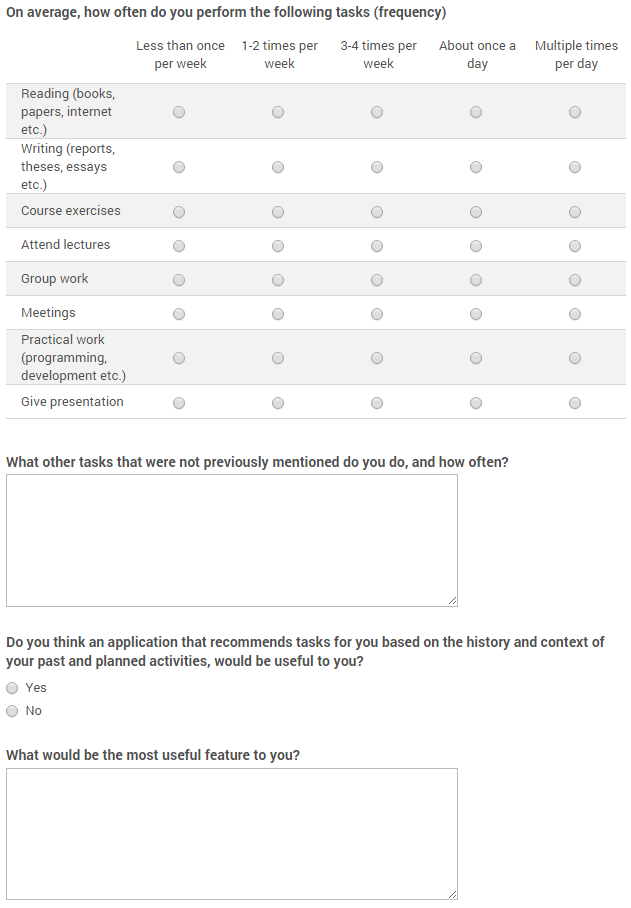
\includegraphics[width=0.8\columnwidth]{appendix/StudentTasks2.PNG}
\caption{Student tasks questionnaire part 2.}
\end{figure}



\chapter{Application GUI}

\begin{figure}[h]
\centering
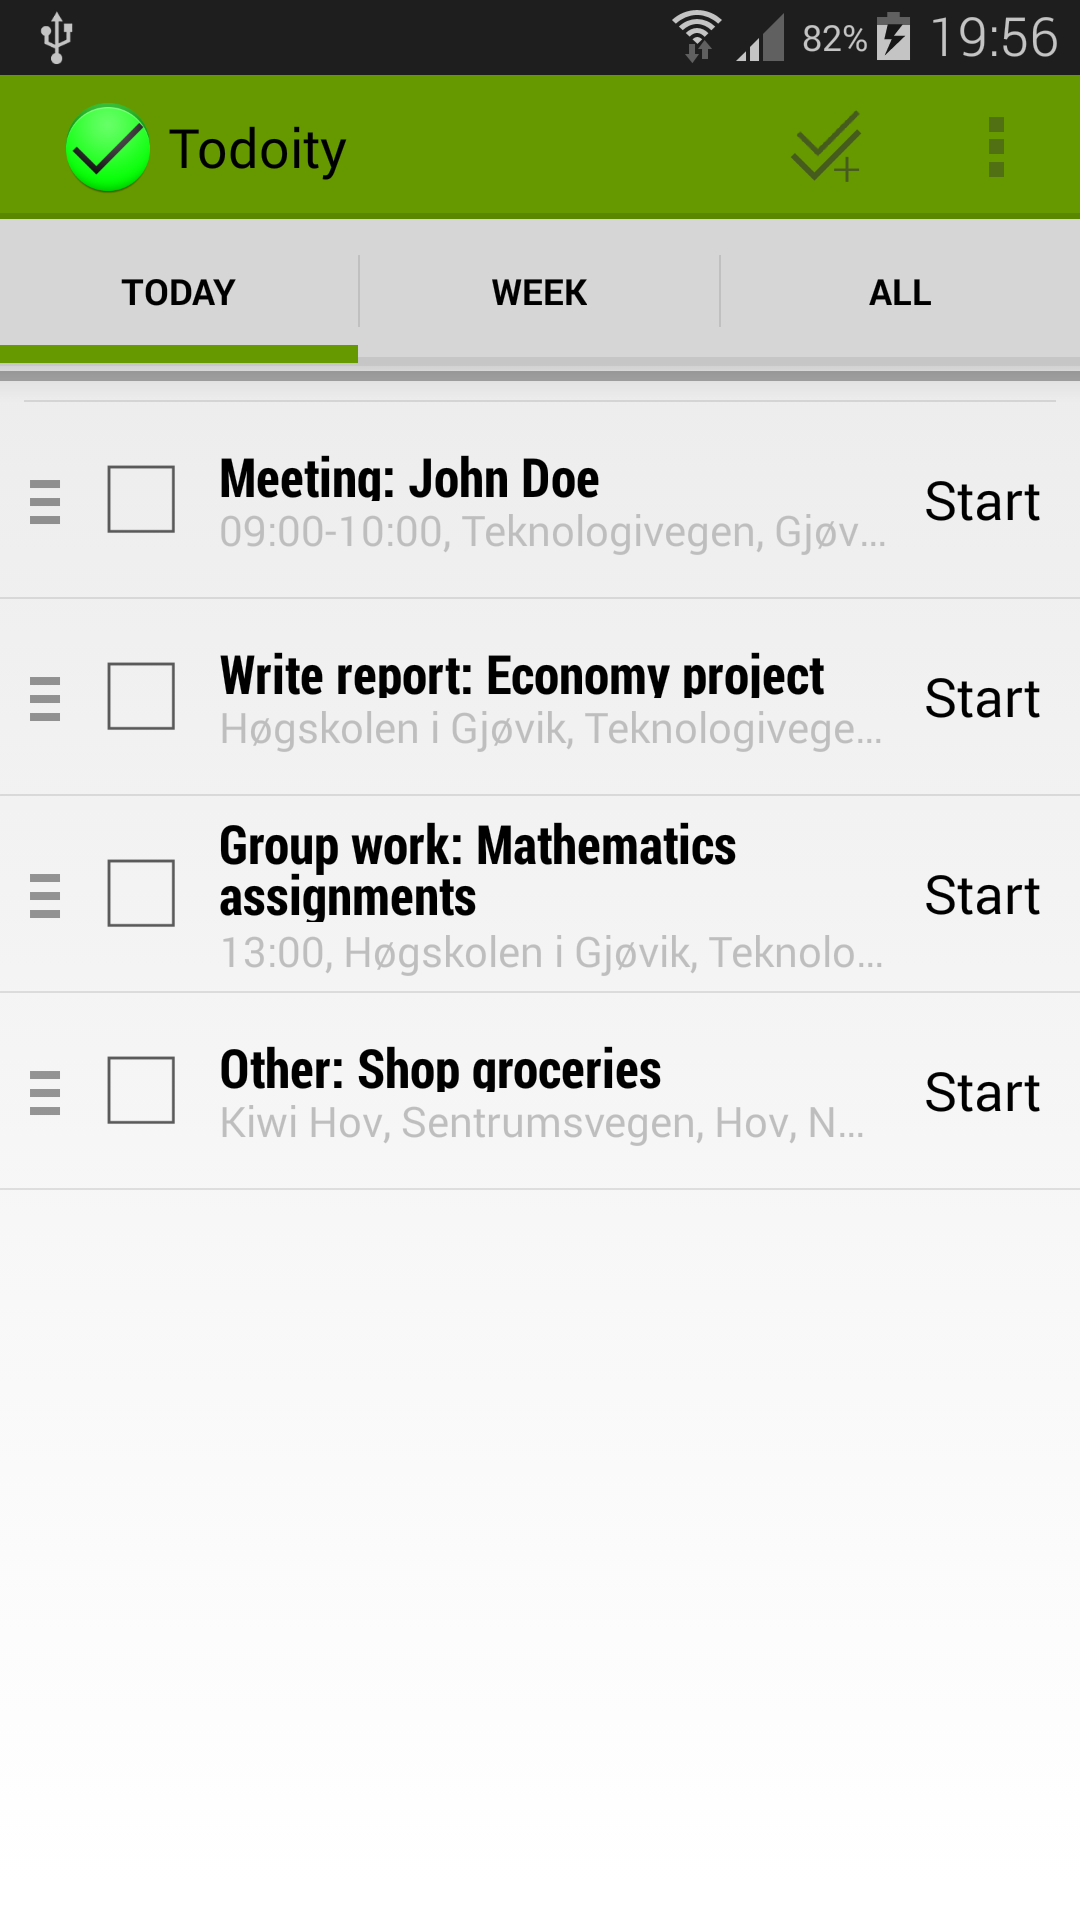
\includegraphics[width=0.25\columnwidth]{appendix/MainScreenToday.PNG}
\caption{Main application screen design showing tasks for ``today''.}
\end{figure}

\begin{figure}[h]
\centering
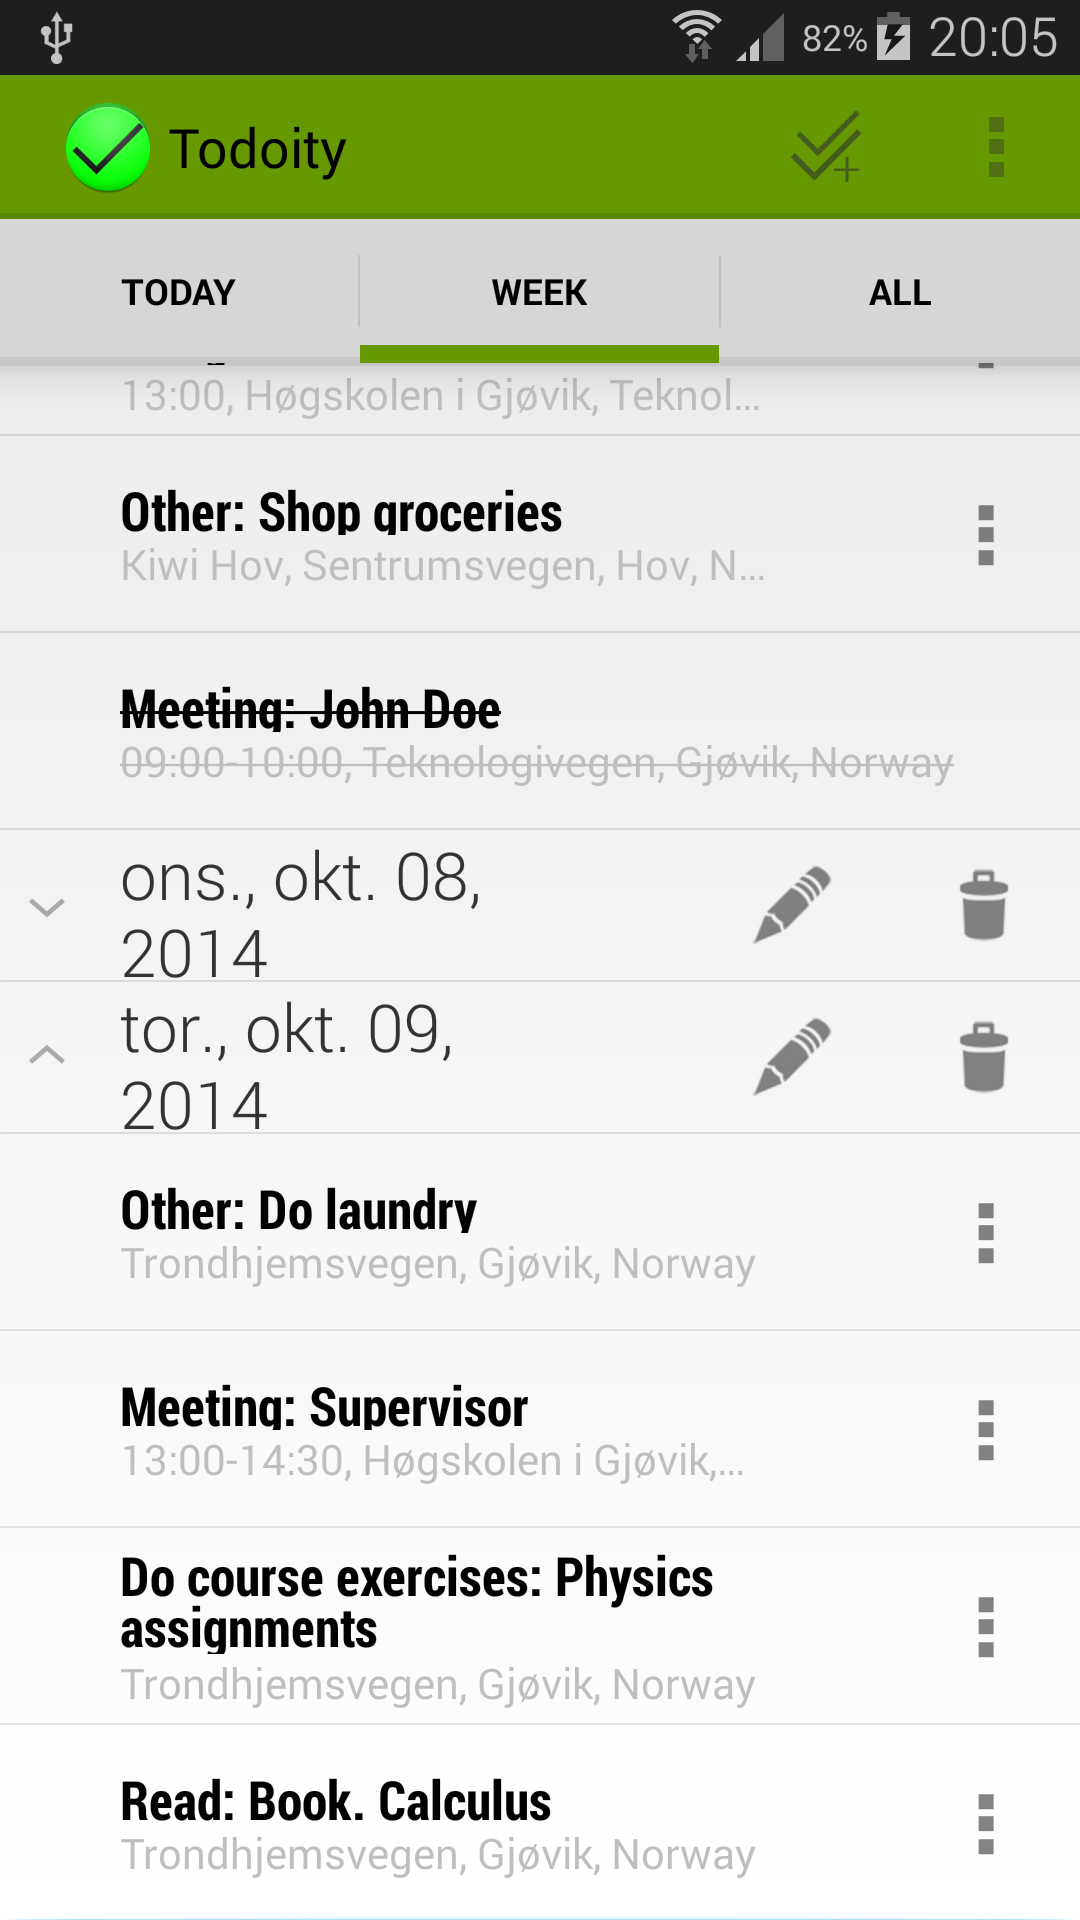
\includegraphics[width=0.25\columnwidth]{appendix/MainScreenWeek.PNG}
\caption{Main application screen design showing tasks for the ``week''.}
\end{figure}



\chapter{Recommender algorithm}

\lstset{ %
  backgroundcolor=\color{white},   % choose the background color
  basicstyle=\ttfamily\scriptsize, % size of fonts used for the code
  breaklines=true,                 % automatic line breaking only at whitespace
  captionpos=b,                    % sets the caption-position to bottom
  commentstyle=\color{green},    % comment style
  keywordstyle=\color{blue},       % keyword style
  stringstyle=\color{red},     % string literal style
}
\lstinputlisting[language=Java, firstline=27]{appendix/Recommender.java}